\section{Overview}

This very basic tutorial provides an introduction to Bayesian inference and Markov chain Monte Carlo (MCMC) algorithms.
The tutorial explains the fundamental concepts of an MCMC algorithm, such as \emph{moves} and \emph{monitors}, which are ubiquitous in every other tutorial.
After the tutorial you should be somewhat familiar with Bayesian inference (\EG what is a prior distribution, posterior distribution, and likelihood function) and MCMC simulation (\EG what are moves and monitors and why do we need them).

\section{A Coin Flipping (Binomial) Model}

We'll begin our exploration of Bayesian inference with a simple coin-flipping model.
In this model, we imagine flipping a coin $n$ times and count the number of heads, $x$; each flip comes up heads with probability $p$.
This model gives rise to the Binomial probability distribution, with parameters $n$ and $p$:
\begin{align*}
P(x \mid n,p) = {n \choose x}p^x(1-p)^{n-x}
\end{align*}
Simple intuition suggests that, given that we observe $x$ heads in $n$ coin tosses, the maximum-likelihood estimate (MLE) of $p$ is simply $\frac{x}{n}$: if we flip a coin 100 times and observe 70 heads, we assume the probability the coin comes up heads is $\frac{70}{100} = 0.7$.
This is indeed the maximum likelihood estimate!

From Bayes' theorem, the \emph{posterior distribution} of $p$ given $x$, $P(p \mid x)$, is:
\begin{align*}
\overbrace{P(p \mid x)}^{\text{posterior distribution}} = \frac{ \overbrace{P(x \mid p)}^{\text{likelihood}} \times \overbrace{P(p)}^{\text{prior}}}{\underbrace{P(x)}_{\text{marginal likelihood}}}
\end{align*}
The take-home message here is that, if we're interested in doing Bayesian inference for the coin flipping model, we need to specify a \emph{likelihood function} and a \emph{prior distribution} for $p$.
In virtually all practical cases, we cannot compute the posterior distribution directly and instead use numerical procedures, such as a Markov chain Monte Carlo (MCMC) algorithm.
Therefore, we will also have to write an MCMC algorithm that samples parameter values in the frequency of their posterior probability.

We'll use a simple beta distribution as a prior on the parameter of the model, $p$.
The beta distribution has two parameters, $\alpha$ and $\beta$ (Figure~\ref{fig:beta_distribution}).
Different choices for $\alpha$ and $\beta$ represent different prior beliefs.
\begin{figure}[h!]
\centering
\fbox{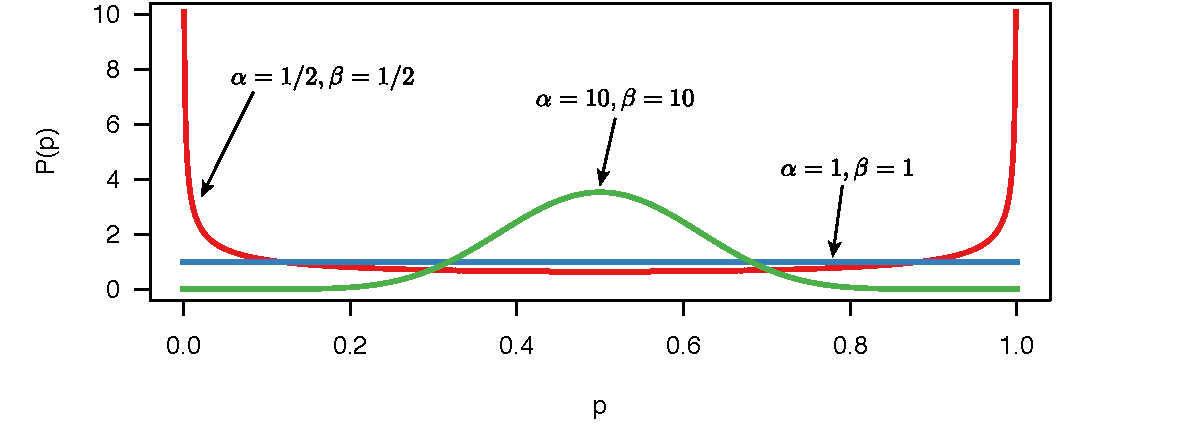
\includegraphics[width=0.7\linewidth,angle=0]{\ResourcePath figures/beta.pdf}}
\label{fig:beta_distribution}
\caption{A beta distribution with two parameters, $\alpha$ and $\beta$. This distribution is used as a prior distribution on the probability parameter $p$ of observing a head. Here we show different curves for the beta distribution when using different parameters.}
\end{figure}


Figure~\ref{fig:binomial_model} shows the graphical model for the binomial model.
This nicely visualizes the dependency structure in the model.
We see that the two parameters $\alpha$ and $\beta$ are drawn in solid squares, representing that these variables are constant.
From these two variables, we see arrows going into the variable $p$.
That simply means that $p$ depends on $\alpha$ and $\beta$.
More specifically, $p$ is a stochastic variable (shown as a solid circle) and drawn from a beta distribution with parameters $\alpha$ and $\beta$.
Then, we have another constant variable, $n$.
Finally, we have the observed data $x$ which is drawn from a Binomial distribution with parameters $p$ and $n$, as can be seen by the arrows going into $x$.
Furthermore, the solid circle of $x$ is shaded which means that the variable has data attached to it.
\begin{figure}[h!]
\centering
\fbox{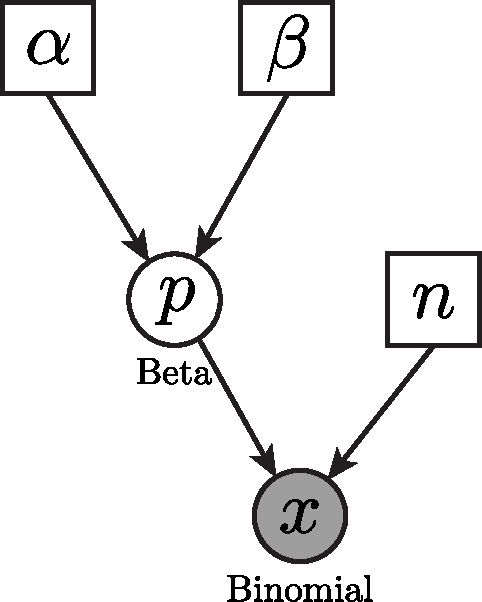
\includegraphics[width=1.8in,angle=0]{\ResourcePath figures/binomial_graphical_model.pdf}}
\label{fig:binomial_model}
\caption{A graphical model for the binomial model.}
\end{figure}



\section{Writing an MCMC from Scratch}

\impmark Make yourself familiar with the example script called \emph{Binomial\_MH\_algorithm.Rev} which shows the code for the following sections. Then, start a new and empty script and follow each step provided in the \colorbox{shadecolor}{blue boxes}.

\subsection{The Metropolis-Hastings Algorithm}
Though \RevBayes implements efficient and easy-to-use Markov chain Monte Carlo algorithms, we'll begin by writing one ourselves to gain a better understanding of the moving parts.
The Metropolis-Hastings MCMC algorithm \citep{Metropolis1953,Hastings1970} proceeds as follows:

\begin{enumerate}
	\item Generate initial values for the parameters of the model (in this case, $p$).
	\item Propose a new value (which we'll call $p^\prime$) for some parameters of the model, (possibly) based on their current values 
	\item Calculate the acceptance probability, $R$, according to:
	\begin{align*}
		R = \text{min}\left\{1, \frac{P(x \mid p^\prime)}{P(x \mid p)} \times \frac{P(p^\prime)}{P(p)} \times \frac{q(p)}{q(p^\prime)} \right\}
	\end{align*}
	\item Generate a uniform random number between 1 and 0. If it is less than $R$, accept the move (set $p = p^\prime$). Otherwise, keep the current value of $p$.
	\item Record the values of the parameters.
	\item Return to step 2 many many times, keeping track of the value of $p$.
\end{enumerate}

\subsection{Reading in the data}
Actually, in this case, we're just going to make up some data on the spot.
Feel free to alter these values to see how they influence the posterior distribution
{\tt \begin{snugshade*}
\begin{lstlisting}    
# Make up some coin flips!
# Feel free to change these numbers
n <- 100 # the number of flips
x <- 63	# the number of heads
\end{lstlisting}
\end{snugshade*}}

\subsection{Initializing the Markov chain}
We have to start the MCMC off with some initial parameter values.
One way to do this is to randomly draw values of the parameters (just $p$, in this case) from the prior distribution.
We'll assume a ``flat'' beta prior distribution; that is, one with parameters $\alpha = 1$ and $\beta = 1$.
{\tt \begin{snugshade*}
\begin{lstlisting}
# Initialize the chain with starting values
alpha <- 1
beta  <- 1
p <- rbeta(n=1,alpha,beta)[1]
\end{lstlisting}
\end{snugshade*}}
\pagebreak
\subsubsection{Likelihood function}
We also need to specify the likelihood function.
We use the binomial probability for the likelihood function. Since the likelihood is defined only for values of $p$ between 0 and 1, we return 0.0 if $p$ is outside this range:
{\tt \begin{snugshade*}
\begin{lstlisting}
# specify the likelihood function
function likelihood(p) {
    if(p < 0 || p > 1)
        return 0

    l = dbinomial(x,p,n,log=false)
    return l
}
\end{lstlisting}
\end{snugshade*}}

\subsubsection{Prior distribution}
Similarly, we need to specify a function for the prior distribution.
Here, we use the beta probability distribution for the prior on $p$:
{\tt \begin{snugshade*}
\begin{lstlisting}    
# specify the prior function
function prior(p) {
    if(p < 0 || p > 1)
        return 0
        
    pp = dbeta(p,alpha,beta,log=false)
    return pp
}
\end{lstlisting}
\end{snugshade*}}


\subsubsection{Monitoring parameter values}
Additionally, we are going to monitor, \IE store, parameter values into a file during the MCMC simulation.
For this file we need to write the column headers:
{\tt \begin{snugshade*}
\begin{lstlisting}
# Prepare a file to log our samples
write("iteration","p","\n",file="binomial_MH.log")
write(0,p,"\n",file="binomial_MH.log",append=TRUE)
\end{lstlisting}
\end{snugshade*}}
(You may have to change the newline characters to \texttt{"$\backslash$r$\backslash$n"} if you're using a Windows operating system.)
We'll also monitor the parameter values to the screen, so let's print the initial values:
{\tt \begin{snugshade*}
\begin{lstlisting}
# Print the initial values to the screen
print("iteration","p")
print(0,p)
\end{lstlisting}
\end{snugshade*}}

\subsection{Writing the MH Algorithm}
At long last, we can write our MCMC algorithm.
First, let us define the frequency how often we print to file (\IE monitor), which is also often called thinning.
If we set the variable \cl{printgen} to 1, then we will store the parameter values every single iteration; if we choose \cl{printgen=10} instead, then only every $10^{th}$ iteration.
{\tt \begin{snugshade*}
\begin{lstlisting}    
printgen = 10
\end{lstlisting}
\end{snugshade*}}
We will repeat this resampling procedure many times (here, 10000), and iterate the MCMC using a \texttt{for} loop:
{\tt \begin{snugshade*}
\begin{lstlisting}    
# Write the MH algorithm
reps = 10000 
for(rep in 1:reps){
\end{lstlisting}
\end{snugshade*}}
(remember to close your \texttt{for} loop at the end).

The first thing we do in the first generation is generate a new value of $p^\prime$ to evaluate.
We'll propose a new value of $p$ from a uniform distribution between 0 and 1.
Note that in this first example we do not condition new parameter values on the current value.
{\tt \begin{snugshade*}
\begin{lstlisting}    
	# Propose a new value of p
	p_prime <- runif(n=1,0.0,1.0)[1]
\end{lstlisting}
\end{snugshade*}}

Next, we compute the proposed likelihood and prior probabilities, as well as the acceptance probability, $R$:
{\tt \begin{snugshade*}
\begin{lstlisting}    
	# Compute the acceptance probability
	R <- ( likelihood(p_prime) / likelihood(p) ) * ( prior(p_prime) / prior(p) )
\end{lstlisting}
\end{snugshade*}}

Then, we accept the proposal with probability $R$ and reject otherwise:
{\tt \begin{snugshade*}
\begin{lstlisting}    
	# Accept or reject the proposal
	u <- runif(1,0,1)[1]
	if(u < R){
		# Accept the proposal
		p <- p_prime
	}
\end{lstlisting}
\end{snugshade*}}

Finally, we store the current value of $p$ in our log file.
Here, we actually check if we want to store the value during this iteration.
{\tt \begin{snugshade*}
\begin{lstlisting}
    if ( (rep % printgen) == 0 ) {
        # Write the samples to a file
        write(rep,p,"\n",file="binomial_MH.log",append=TRUE)
        # Print the samples to the screen
        print(rep,p)
    }
} # end MCMC\end{lstlisting}
\end{snugshade*}}


\subsection{Visualizing the samples of an MCMC simulation}

Below we show an example of the obtained output in \Tracer.
Specifically, Figure~\ref{fig:mcmc_samples} shows the sample trace (left) and the estimated posterior distribution of $p$ (right).
There are other parameters, such as the posterior mean and the 95\% HPD (highest posterior density) interval, that you can obtain from \Tracer.
\begin{figure}[h!]
\centering
\fbox{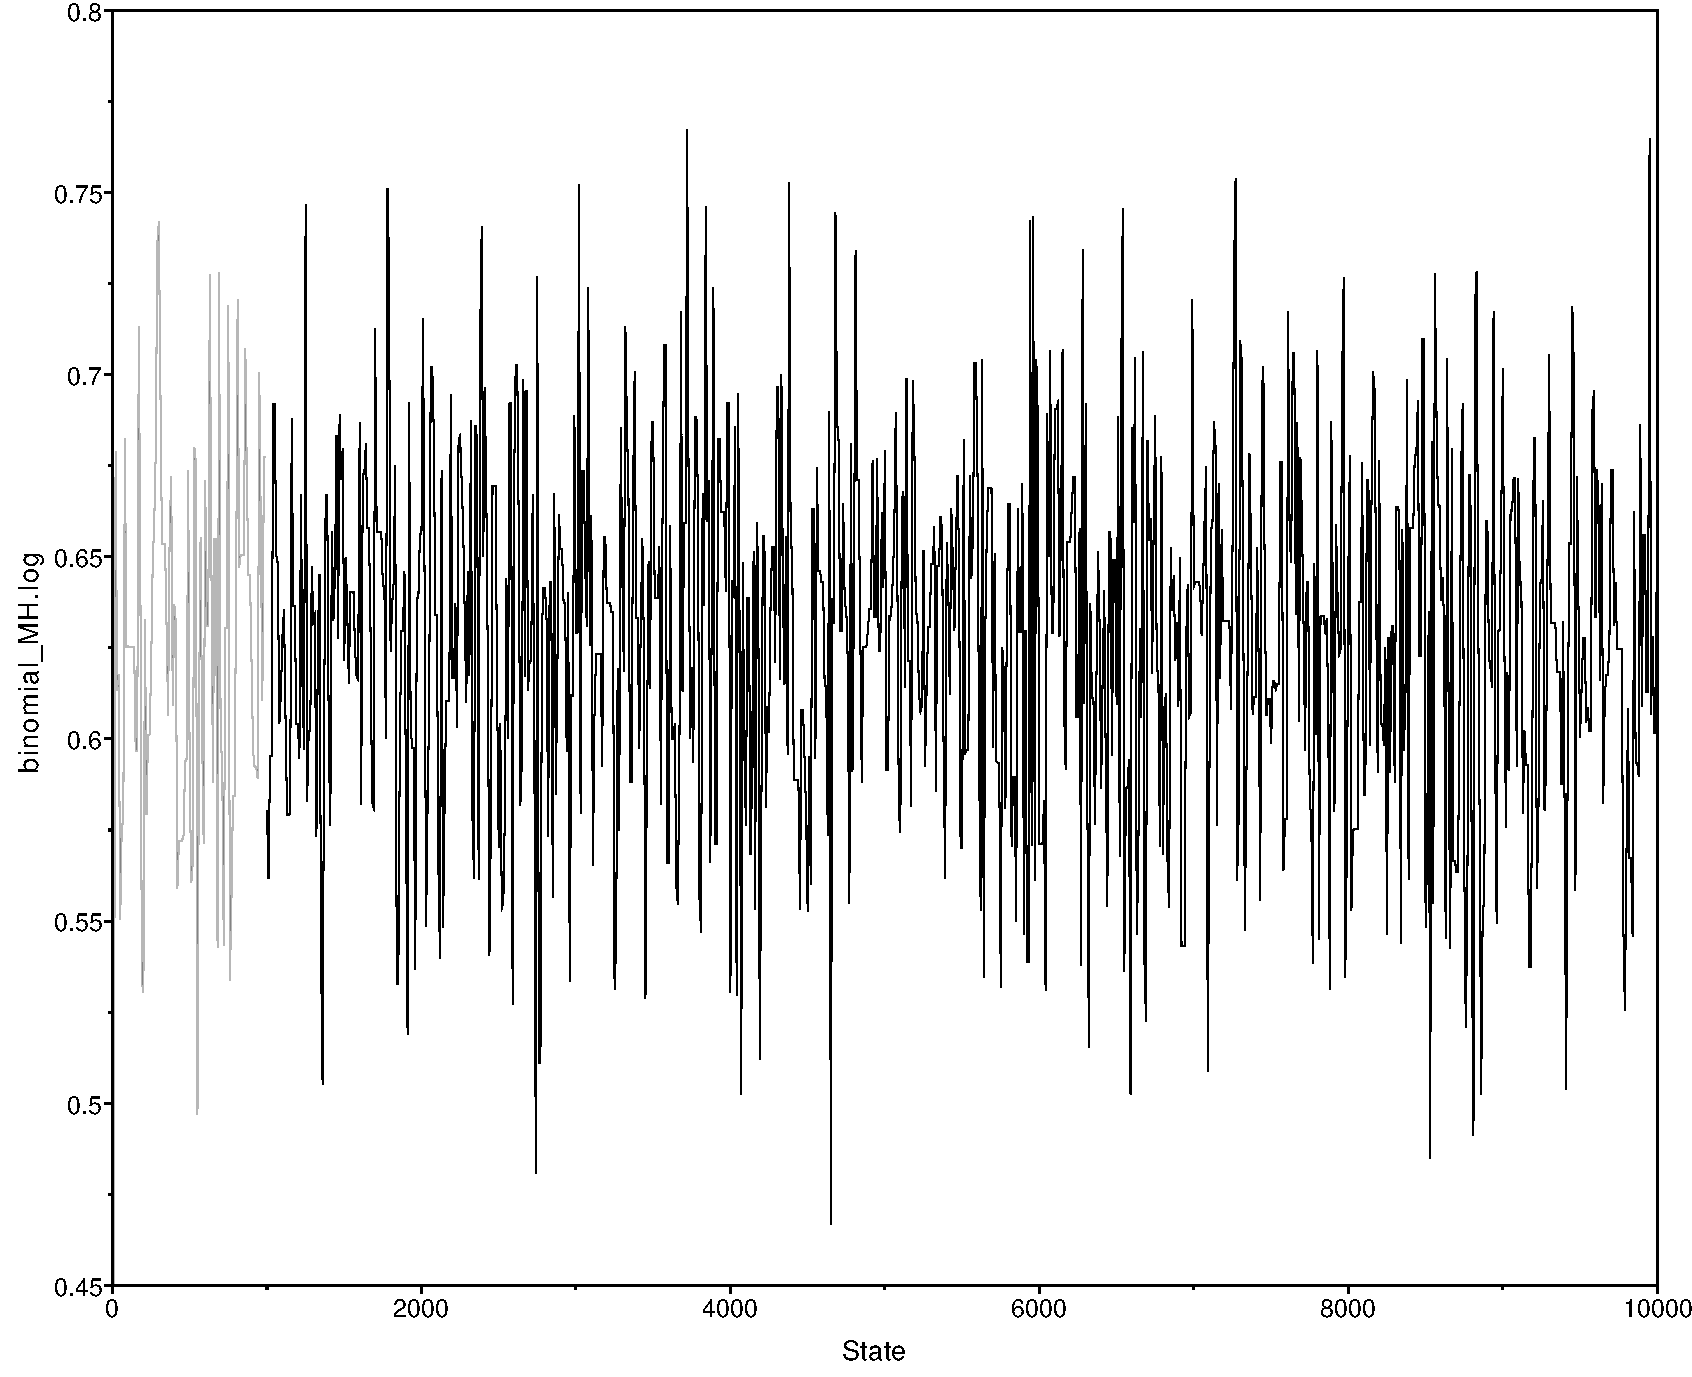
\includegraphics[width=0.45\linewidth,angle=0]{\ResourcePath figures/binomial_MCMC_Trace.pdf}
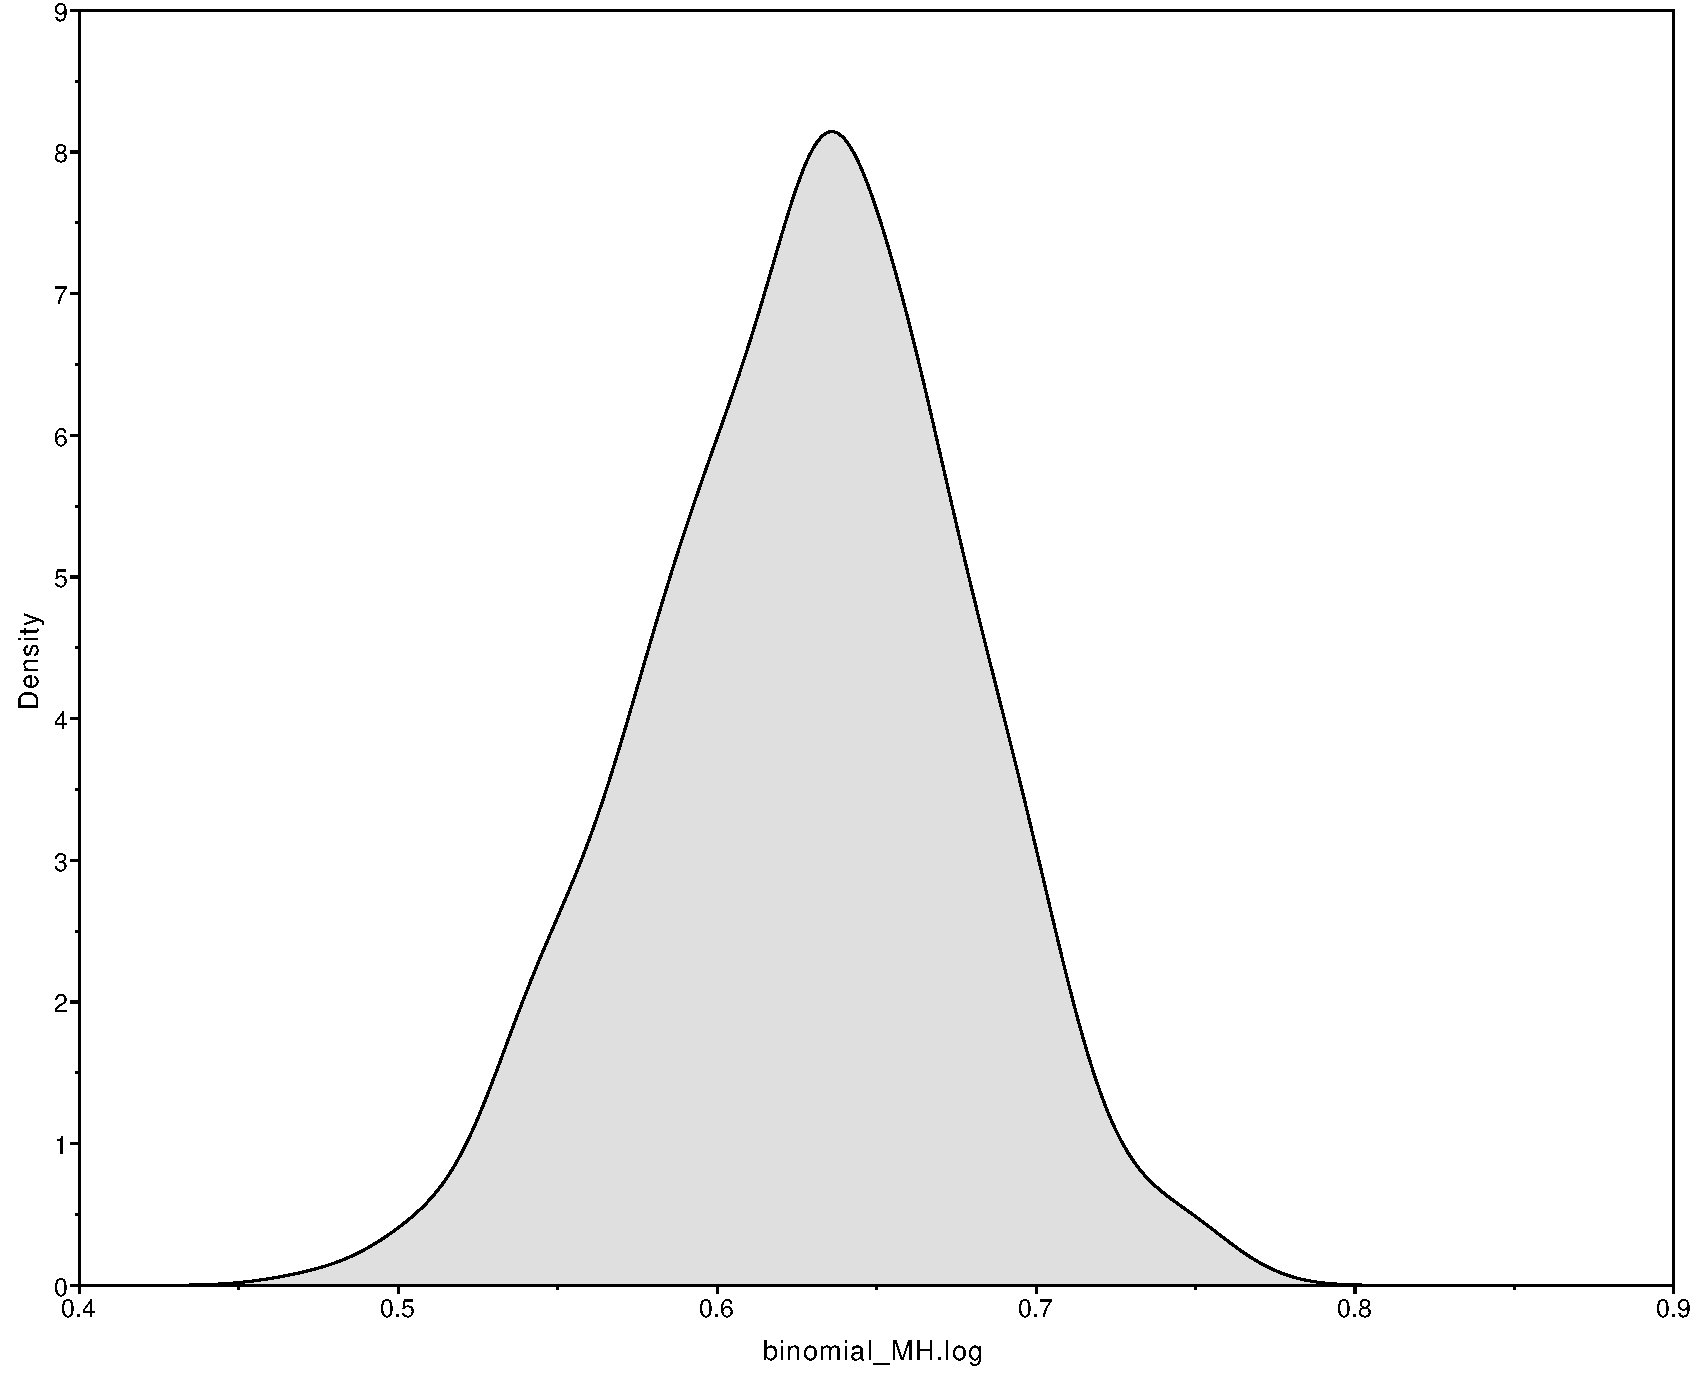
\includegraphics[width=0.45\linewidth,angle=0]{\ResourcePath figures/binomial_MCMC_distribution.pdf}}
\label{fig:mcmc_samples}
\caption{Left: The \emph{Trace} of sample from an MCMC simulation. Right: The approximated posterior probability distribution for $p$.}
\end{figure}

\section{More on Moves: Tuning and weights}

In the previous example we hard coded a single move updating the variable $p$ by drawing a new value from a uniform(0,1) distribution.
There are actually many other ways how to propose new values; some of which are more efficient than others.

First, let us rewrite the MCMC loop so that we use instead a function, which we call \cl{move\_uniform} for simplicity, that performs the move:
{\tt \begin{snugshade*}
\begin{lstlisting}    
for (rep in 1:reps){
    
    # call uniform move
    move_uniform(1)
    
    if ( (rep % printgen) == 0 ) {
        # Write the samples to a file
        write(rep,p,"\n",file="binomial_MH.log",append=TRUE)
    }

} # end MCMC
\end{lstlisting}
\end{snugshade*}}
This loop looks already much cleaner.

\subsection{Uniform move}
Now we need to actually write the \cl{move\_uniform} function.
We mostly just copy the code we had before into a dedicated function
{\tt \begin{snugshade*}
\begin{lstlisting}    
function move_uniform( Natural weight) {

    for (i in 1:weight) {
        # Propose a new value of p
        p_prime <- runif(n=1,0.0,1.0)[1]

        # Compute the acceptance probability
        R <- ( likelihood(p_prime) / likelihood(p) ) * ( prior(p_prime) / prior(p) )
    
        # Accept or reject the proposal
        u <- runif(1,0,1)[1]
        if (u < R){
            # Accept the proposal
            p <- p_prime
        } else {
            # Reject the proposal
            # (we don't have to do anything here)
        }
    }
    
}
\end{lstlisting}
\end{snugshade*}}
There are a few things to consider in the function \cl{move\_uniform}.
First, we do not have a return value because the move simply changes the variable $p$ if the move is accepted.
Second, we expect an argument called \cl{weight} which will tell us how often we want to use this move.
Otherwise, this function does exactly the same what was inside the for loop previously.

(Note that you need to define this function before the for loop in your script).


\subsection{Sliding-window move}
As a second move we will write a sliding-window move.
The sliding-window moves propose an update by drawing a random number from a uniform distribution and then adding this random number to the current value (\IE centered on the previous value).
{\tt \begin{snugshade*}
\begin{lstlisting}    
function move_slide( RealPos delta, Natural weight) {

    for (i in 1:weight) {
        # Propose a new value of p
        p_prime <- p + runiform(n=1,-delta,delta)[1]

        # Compute the acceptance probability
        R <- ( likelihood(p_prime) / likelihood(p) ) * ( prior(p_prime) / prior(p) )
    
        # Accept or reject the proposal
        u <- runif(1,0,1)[1]
        if (u < R) {
            # Accept the proposal
            p <- p_prime
        } else {
            # Reject the proposal
            # (we don't have to do anything here)
        }
    }
    
}
\end{lstlisting}
\end{snugshade*}}
In addition to the weight of the move, this move has another argument, \cl{delta}.
The argument \cl{delta} defines the width of the uniform window from which we draw new values.
Thus, if \cl{delta} is large, then the proposed values are more likely to be very different from the current value of $p$.
Conversely, if \cl{delta} is small, then the proposed values are more likely to be very close to the current value of $p$.

\impmark Experiment with different values for \cl{delta} and check how the effective sample size (ESS) changes.

There is, a priori, no good method for knowing what values of \cl{delta} are most efficient.
However, there are some algorithms implemented in \RevBayes, called \emph{auto-tuning}, that will estimate good values for \cl{delta}.

\subsection{Scaling move}
As a third and final move we will write a scaling move.
The scaling move proposes an update by drawing a random number from a uniform(-0.5,0.5) distribution, exponentiating the random number, and then multiplying this scaling factor by the current value.
An interesting feature of this move is that it is not symmetrical and thus needs a Hastings ratio.
The Hastings ratio is rather trivial in this case, and one only needs to multiply the acceptance rate by the scaling factor.
{\tt \begin{snugshade*}
\begin{lstlisting}    
function move_scale( RealPos lambda, Natural weight) {

    for (i in 1:weight) {
        # Propose a new value of p
        sf <- exp( lambda * ( runif(n=1,0,1)[1] - 0.5 ) )
        p_prime <- p * sf

        # Compute the acceptance probability
        R <- ( likelihood(p_prime) / likelihood(p) ) * ( prior(p_prime) / prior(p) ) * sf
    
        # Accept or reject the proposal
        u <- runif(1,0,1)[1]
        if (u < R){
            # Accept the proposal
            p <- p_prime
        } else {
            # Reject the proposal
            # (we don't have to do anything here)
        }
    }
    
}
\end{lstlisting}
\end{snugshade*}}
As before, this move has a tuning parameter called \emph{lambda}.

\begin{framed}
The sliding-window and scaling moves are very common and popular moves in \RevBayes.
The code examples here are actually showing the exact same equation as implemented internally.
It will be very useful for you to understand these moves.	
\end{framed}

\pagebreak

However, this MCMC algorithm is \emph{very} specific to our binomial model and thus hard to extend (also it's pretty inefficient!).


\section{The Metropolis-Hastings Algorithm with the \emph{Real} \RevBayes}
We'll now specify the exact same model in \Rev using the built-in modeling functionality.
It turns out that the \Rev code to specify the above model is extremely simple and similar to the one we used before.
Again, we start by ``reading in'' (\emph{i.e.}, making up) our data.

{\tt \begin{snugshade*}
\begin{lstlisting}    
# Make up some coin flips!
# Feel free to change these numbers
n <- 100 # the number of flips
x <- 63	# the number of heads
\end{lstlisting}
\end{snugshade*}}

Now we specify our prior model.
{\tt \begin{snugshade*}
\begin{lstlisting}    
# Specify the prior distribution
alpha <- 1
beta  <- 1
p ~ dnBeta(alpha,beta)
\end{lstlisting}
\end{snugshade*}}

One difference between \RevBayes and the MH algorithm that we wrote above is that many MCMC proposals are already built-in, but we have to specify them \emph{before} we run the MCMC.
We usually define (at least) one move per parameter immediately after we specify the prior distribution for that parameter.

{\tt \begin{snugshade*}
\begin{lstlisting}    
# Define a move for our parameter, p
moves[1] = mvSlide(p,delta=0.1,weight=1)
\end{lstlisting}
\end{snugshade*}}

Next, our likelihood model.
{\tt \begin{snugshade*}
\begin{lstlisting}    
# Specify the likelihood model
k ~ dnBinomial(p, n)
k.clamp(x)
\end{lstlisting}
\end{snugshade*}}

We wrap our full Bayesian model into one model object (this is a convenience to keep the entire model in a single object, and is more useful when we have very large models):
{\tt \begin{snugshade*}
\begin{lstlisting}    
# Construct the full model
my_model = model(p)
\end{lstlisting}
\end{snugshade*}}

We use ``monitors'' to keep track of parameters throughout the MCMC.
The two kinds of monitors we use here are the \texttt{mnModel}, which writes parameters to a specified file, and the \texttt{mnScreen}, which simply outputs some parts of the model to screen (as a sort of progress bar).
{\tt \begin{snugshade*}
\begin{lstlisting}    
# Make the monitors to keep track of the MCMC
monitors[1] = mnModel(filename="binomial_MCMC.log", printgen=10, separator = TAB)
monitors[2] = mnScreen(printgen=100, p)
\end{lstlisting}
\end{snugshade*}}

Finally, we assemble the analysis object (which contains the model, the monitors, and the moves) and execute the run using the \texttt{.run} command:
{\tt \begin{snugshade*}
\begin{lstlisting}    
# Make the analysis object
analysis = mcmc(my_model, monitors, moves)

# Run the MCMC
analysis.run(100000)

# Show how the moves performed
analysis.operatorSummary()
\end{lstlisting}
\end{snugshade*}}
\impmark Open the resulting \texttt{binomial\_MCMC.log} file in \texttt{Tracer}.
Do the posterior distributions for the parameter $p$ look the same as the ones we got from our first analysis?

Hopefully, you'll note that this \Rev model is substantially simpler and easier to read than the MH algorithm script we began with.
Perhaps more importantly, this \Rev analysis is \emph{orders of magnitude} faster than our own script, because it makes use of extremely efficient probability calculations built-in to \RevBayes (rather than the ones we hacked together in our own algorithm).


\bibliographystyle{sysbio}
\bibliography{\GlobalResourcePath refs}





